\chapter{Результаты}

\section{Сравнение методов первого и второго порядка}
Сравнение методов различных порядков проводилось на модельных задачах в областях с нулевым коэффициентом поглощения. Это позволяет исследовать численную диффузию лучей в отсутствии затухания.

\subsection{Решение уравнения в одном направлении}
Сравнение методов проводилось на следующей задаче. Рассматривалась
геометрическая область, куб со стороной $a = 2$. 
В центре области находится
крест, состоящий из пяти одинаковых кубиков со стороной $b = 0.2$ (см. рис. \ref{fig:6}).
\begin{figure}[ht!]
\centering
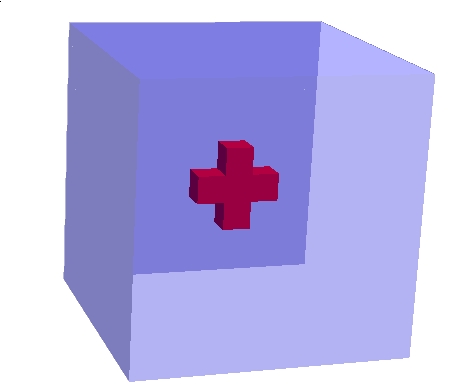
\includegraphics[width = 0.4\textwidth]{cross.png}
\caption{Расчетная область}
\label{fig:6}
\end{figure}
Коэффициент поглощения в области равен $\varkappa_1=0$, а внутри креста --- $\varkappa_2 = 100$. Равновесная интенсивность в центральной области $1$, а в окружающей среде --- $0$. Решение строилось вдоль одного направления, $\omega = (0,0,1)$ на сетке с $415625$ тетраэдрами и $76247$ вершинами. Изучалось решение на выходной грани куба. 
\begin{figure}[ht!]
\centering
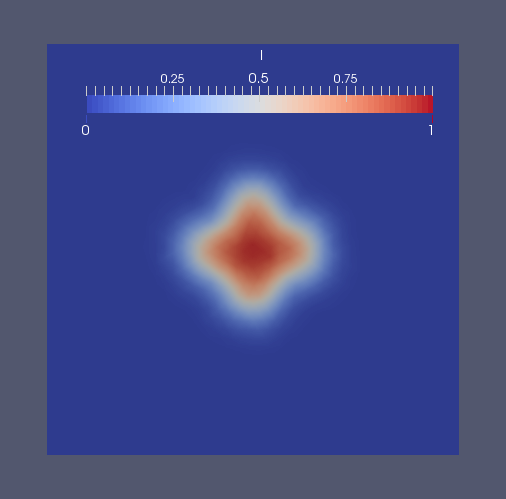
\includegraphics[width = 0.3\textwidth]{1ord.png}%
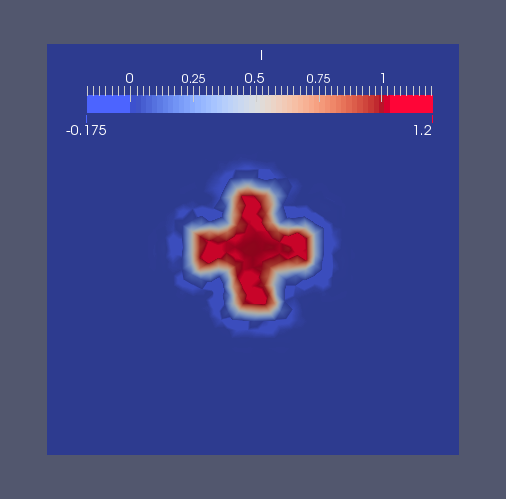
\includegraphics[width = 0.3\textwidth]{2nolim.png}%
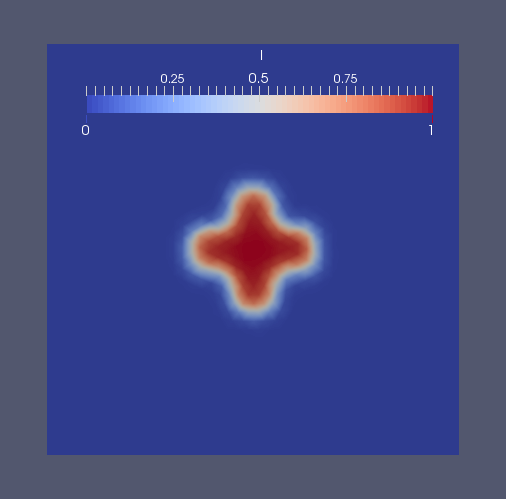
\includegraphics[width = 0.3\textwidth]{2wilim.png}
\caption{Сравнение решений методами первого порядка (слева), второго (в центре) и второго с ограничителем(справа)}
\label{fig:7}
\end{figure}

Точное решение должно представлять собой крест с интенсивностью $1 -
e^{b\varkappa_2} = 1-e^{-20} \approx 1$. Можно видеть (см. рис. \ref{fig:7}), что для первого порядка диффузия достаточно велика, второй порядок без ограничителя отклоняется от допустимых пределов $I \in [0, 1]$ на $20 \%$.
\subsection{Сравнение плотности излучения}
На той же самой задаче изучалась плотность излучения в центральном сечении куба, но коэффициенты поглощения изменились следующим образом: $\varkappa_1 = 10$, $\varkappa_2 = 1$. Использовались 170 направлений из квадратурной формулы Лебедева \cite{lebedev_1999}. 

\begin{figure}[ht!]
\centering
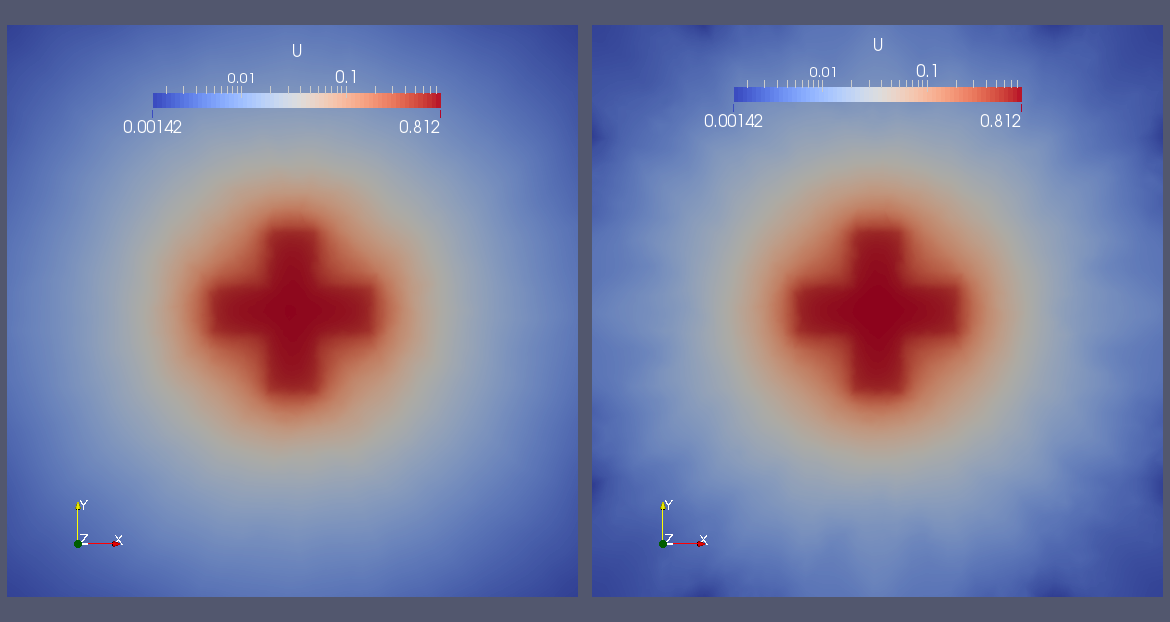
\includegraphics[width = \textwidth]{U2vs1.png}
\caption{Сравнение плотности излучения в центральном сечении куба. Слева первый порядок, справа --- второй}
\label{fig:9}
\end{figure}

\begin{figure}[ht!]
\centering
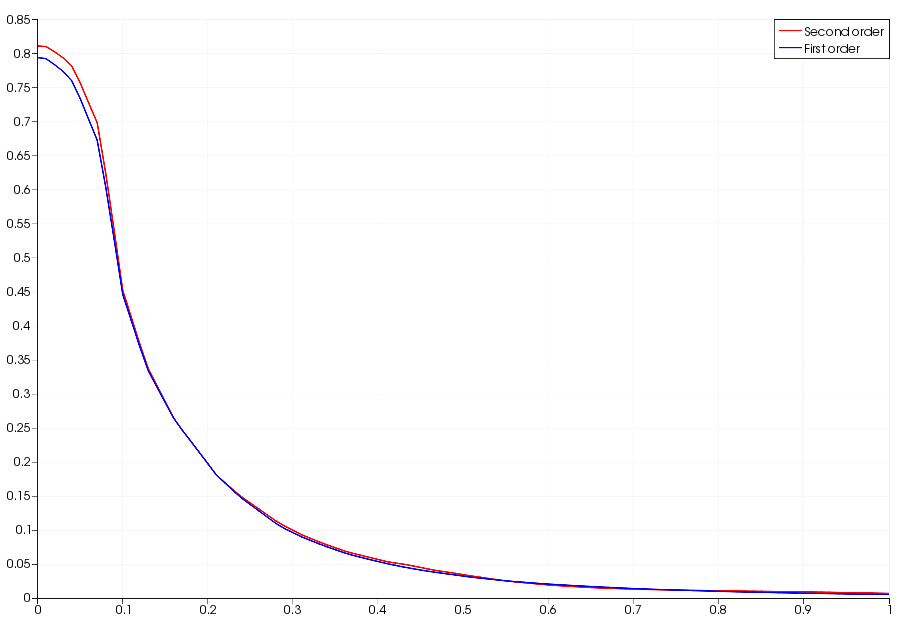
\includegraphics[width = .5\textwidth]{U2vs1Line.png}
\caption{Плотность излучения вдоль оси $Oz$. Красная линия соответствует методу второго порядка, синяя - первого}
\label{fig:10}
\end{figure}
Сравнение плотности излучения (см рис. \ref{fig:9} и \ref{fig:10}) показывает схожие результаты: интенсивность в центре куба в методе второго порядка на $\approx 2 \%$ больше, чем в случае метода первого порядка. В случае метода второго порядка \ref{fig:9} более выражен <<эффект луча>>, в то время как в методе первого порядка этот эффект сглажен за счет численной диффузии. 

\section{Сравнение методов первого и второго порядка с одинаковым количеством узловых точек}

Корректное сравнение методов разного порядка аппроксимации необходимо проводить при одинаковом количестве узловых точек, иначе метод второго порядка априори оказывается точнее. Использовалась кусочно-линейная модификация \eqref{eq:piecewiselinear}.

Расчетная область состояла из двух концентрических сфер с центром в точке $(0,0,0)$, внешняя радиусом $R = 5$, а внутренняя --- $r = 0.35$ (см. рис. \ref{fig:11}). Коэффициент поглощения в области между сферами равен $\varkappa_1 = 0$, а внутри меньшей сферы --- $\varkappa_2 = 10$. Равновесная интенсивность в центральной области $I_{p,2} = 1$, а в окружающей среде --- $I_{p,1} = 0$. 
\begin{figure}[ht!]
\centering
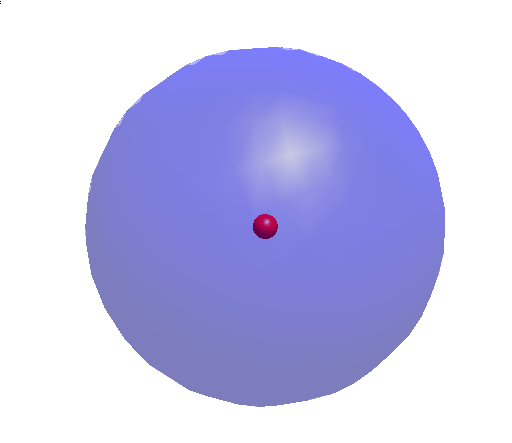
\includegraphics[width = 0.5\textwidth]{sphere.png}
\caption{Расчетная область в случае сравнения методов первого и второго порядка с одинаковым количеством узловых точек}
\label{fig:11}
\end{figure}
Решение строилось вдоль одного направления $\omega = (1, 0, 0)$ на сетке с $387736$ тетраэдрами и $70705$ вершинами. Изучалось решение в центральном сечении. 
\begin{figure}[ht!]
\centering
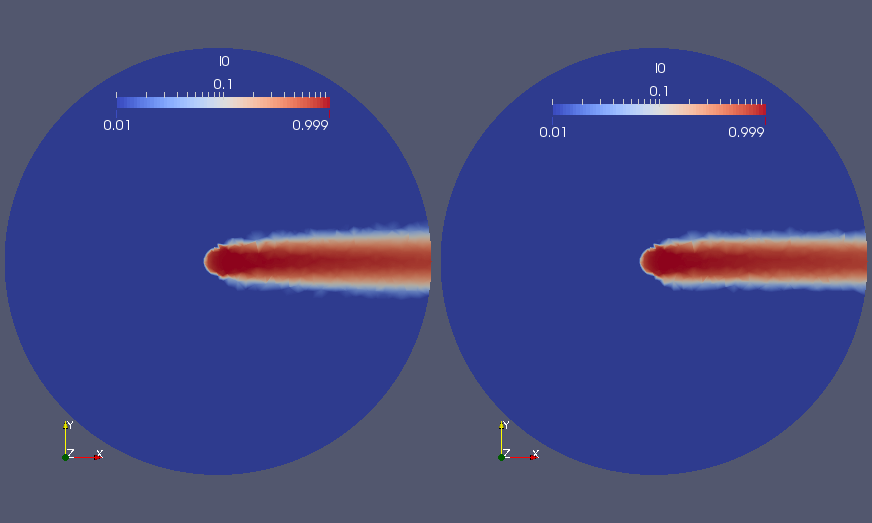
\includegraphics[width = 0.7\textwidth]{2vs15.png}
\caption{Диффузия луча в методе первого (слева) и второго (справа) порядка при одинаковом количестве узловых точек}
\label{fig:12}
\end{figure}

Увеличение количества узловых точек делает метод первого порядка практически таким же точным, как и метод второго порядка, однако численное рассеяние луча имеет различный качественный характер в обоих случаях (см. рис. \ref{fig:12}). В случае метода второго порядка оно практически не меняется вдоль луча, в то время как для метода первого порядка оно растет пропорционально корню удаления от источника ($\Delta y^2 \sim x$), как и должно быть в случае метода первого порядка. 

\section{Моделирование спектра излучения молодой звезды}
Уравнение переноса решалось по результатом газодинамического моделирования взаимодействия магнитного поля молодой звезды типа Т-Тельца с ее аккреционным диском, проведенного в работе \cite{rom_2009}. В численном газодинамическом моделировании наблюдался так называемый конический ветер с углом раствора около $45^\circ$ (см. изоповерхность плотности на рис. \ref{fig:15} справа). 
\begin{figure}[ht!]
\centering
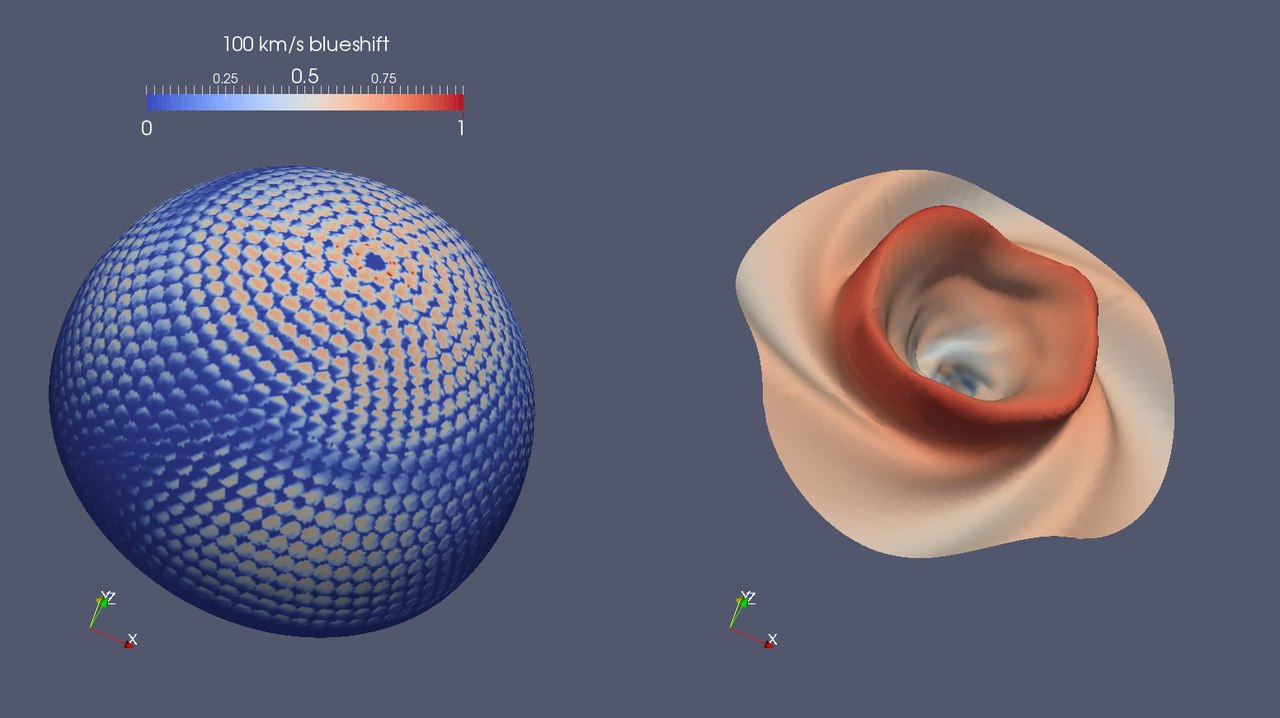
\includegraphics[width = 0.7\textwidth]{star.jpg}
\caption{Слева интенсивности излучения звезды в различных направлениях на частоте, соответствующей синему смещению в $180 \text{ км/с}$. Справа - изоповерхность плотности вещества}
\label{fig:15}
\end{figure}

Уравнение переноса решалось с использованием $1091$ направления и $64$ частотных групп, соответствующих доплеровскому смещению от $-600 \text{ км/с}$ до $600 \text{ км/с}$. Так как интегральные характеристики излучения в этой задаче не важны, вместо квадратурной формулы Лебедева использовалась плотная сетка направлений, равномерная по полярному углу $\theta$ и при каждом фиксированном $\theta$ равномерная по азимутальному углу $\varphi$. Мелкость сетки выбирается так, чтобы лучи заполняли сферу направлений практически без зазоров.

Источником излучения служит сама звезда, находящаяся в центре области. Спектр излучения звезды соответствует линии водорода $\text{H}\alpha$, испытывающей тепловое доплеровское уширение с температурой $T = 4.6 \cdot 10^6 \text{ K}$. Равновесное излучение в окружающем звезду пространстве считается отсутствующим. Коэффициенты поглощения рассчитывались в приближении локального термодинамического равновесия. В коэффициенте поглощения учитывалось смещение частоты поглощения из-за движения вещества.
 
\begin{figure}[ht!]
\centering
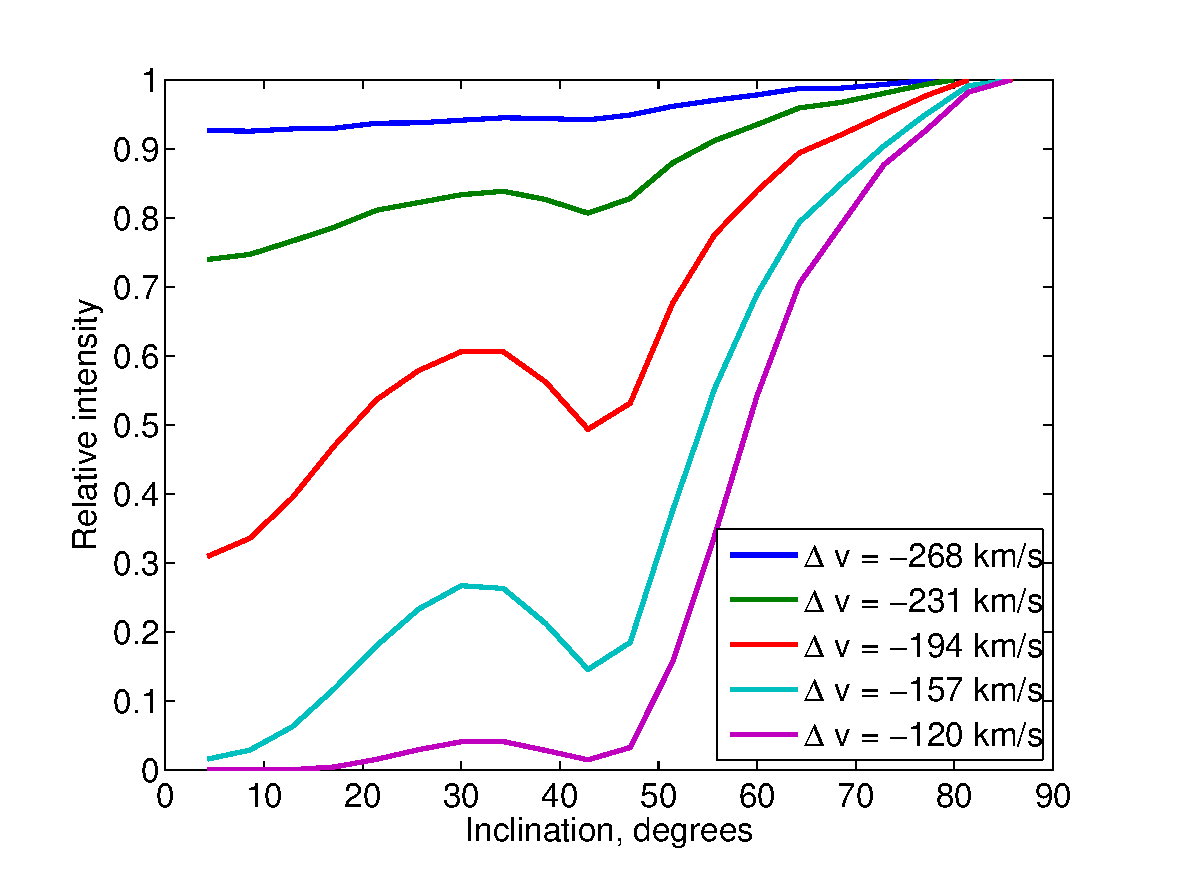
\includegraphics[width = 0.6\textwidth]{varinc.eps}
\caption{Средняя за период обращения относительная интенсивность излучения на разных частотах в зависимости от угла наклонения Земли по отношению к плоскости вращения звезды}
\label{fig:16}
\end{figure}
На частоте, соответствующей синему смещению (вещество движется к наблюдателю) в $180 \text{ км/с}$, наблюдается значительное поглощение в тех направлениях, которые проходят через область конического ветра. На рисунке \ref{fig:15} слева изображено объединение интенсивностей вдоль каждого из исследуемых направлений. На рисунке \ref{fig:16} изображена относительная интенсивность за период обращения звезды в зависимости от угла наклонения (угла, под которым Земля видна из плоскости вращения звезды). Значительное поглощение можно наблюдать для спектральных групп, соответствующих скоростям $\Delta v = -194 \text{ км/с}$ и $\Delta v = -157 \text{ км/с}$ при угле наклонения $45^\circ$.